% * How many of original goals were achieved? Proved to have been achieved
% * Did the program really work?
% *! Credit for interesting conclusion

% ************
% Should have: 
% 	intro
% 	content
% 	summary
% ************

% What I want to say
%
% Questions to answer:
% * Are Distributed Hash Tables viable data stores for a distributed search engine?
% * Do they scale with size?
% * How do Chord and Pastry compare?
%
% Discuss how started with factorial design with factors of nodes and rate.
% Found doesn't vary over length of run, so any run viable.
% All data from three separate runs.
%
% What looked at was latency and success rate.
% 
% Findings to comment on:
% * Why is Chord so much slower than Pastry?
% * Why does Chord has such a low yield rate compared to Pastry
%
% Conclude
% * Does it work for search engine?

\chapter{Evaluation}
In this chapter I look at whether or not Distributed Hash Table are suitable back end data stores for distributed search engines of the specific kind I set out to build. We will furthermore look at how the performance of Chord and Pastry compares in terms of latency and also briefly discuss the benefits of the proximity heuristic used in routing by Pastry. 

\section{What to evaluate}
% Questions to answer:
% * Are Distributed Hash Tables viable data stores for a distributed search engine?
% * Do they scale with size?
% * How do Chord and Pastry compare?
% What looked at was latency and success rate.
My main concern in this evaluation is if Distributed Hash Tables can be used as data stores for my distributed search engine. The determining factor will be the latency between issuing a key lookup request and receiving its value. Therefore, the only dependent variable I will look at in depth is latency.
The latency directly affects the response time as it is seen by the end users using the search engine and also directly affects to what extent predictive searches are possible as there are latency requirements associated with something being perceived as real-time.
Latency also affects whether or not my proposed \emph{link record} scheme can be used, and, by extension, if predictive and fuzzy searches on top of Distributed Hash Tables can be done since link records in my implementation is a prerequisite for that to be possible.
I also want to evaluate the success rate of requests as failed requests would need to be repeated, and therefore directly affect the latency.
It is also interesting to look at how the performance, again in terms of latency, is affected by the number of nodes in the Distributed Hash Table.
In evaluating if Distributed Hash Tables are viable data stores for my search engine it is also interesting to compare the performance of Chord and Pastry to see if one is a better choice than the other.

I will not look at the overhead of maintaining routing state as it is negligible for a well tuned Distributed Hash Table \cite{myths} and does not affect my dependent variable.

\section{Experimental design}
% Discuss how started with factorial design with factors of nodes and rate.
% Found doesn't vary over length of run, so any run viable.
% All data from three separate runs.
I ran my Distributed Hash Tables on machines in the Planet-Lab network. With that in mind, the variables I was able to control were the number of machines participating in the system, the number of Distributed Hash Table nodes running on each machine, and the rate of requests in the network.

In my tests I used all the machines available to me to give some scale to the experiments, and limited the experimental factors to the number of nodes run on each machine and the rate at which requests were issued.

My experiments follow a factorial design where both node count and rate varied between 1 and 16 in powers of two. Since the theory behind Distributed Hash Tables indicate that the number of routing hops is proportional to the logarithm of the number of nodes in the system, and the number of hops directly affect our dependent variable latency, increasing the number of hops in powers of two is reasonable. Doing the same for the rate allows us higher resolution into the lower rates while still giving us data from a wide range of rates to evaluate.
Each configuration was run at three different occasions for both Chord and Pastry, and the log files for all three runs with the same configurations were then used to give the following results.

\subsection{Experimental pattern}
Each experimental run followed a predefined pattern:
\begin{enumerate}
\item I would ensure that the correct number of nodes was running and allow 3 minutes for routing state to adjusted itself if the node count was not correct. 3 minutes was chosen as it gave me high confidence that the routing state would be up-to-date, given the high rate at which the nodes were configured to update their routing state.
\item Each machine would clear old logs and start logging.
\item The experiment would start and each machine in the distributed search engine, each hosting the same number of Distributed Hash Table nodes, would issue requests to its locally hosted nodes at a rate specified for that particular experimental run.
\item After a successfully completed run, there would be a cool down period with continued logging where requests taking slightly longer than permitted would be allowed to finish. Logging would then stop and the logs from the individual machines would be collected at the central hub node.
\item The logs were then downloaded from the central hub to my personal machine for safekeeping and analysis.
\item The process was then repeated for different experimental parameters.
\end{enumerate}

\section{Effects of Planet-Lab}
As mentioned, my experiments ran on top of machines provided by Planet-Lab. I was allowed to use up to 100 machines, but never managed to have them all running at the same time.

Using Planet-Lab as a test bed gave me several benefits: the machines at my disposal had a high geographical spread and varied greatly in what computational resources they provided. Depending on the time of day the computational load on the machines would also vary and not only that, but I would have a different subset of the machines available for testing from day to day.
This provided an excellent foundation for testing Distributed Hash Tables which are meant to be able to cope with high node churn and machines with widely different capabilities and additionally abstracts away the specific topology used for the experiments.

While Planet-Lab provides an interesting test bed, the randomness with which computational resources are available makes it impossible to accurately repeat experiments. Rerunning an experiment would invariably give a slightly different result.
To work with Planet-Lab's strengths and not against it, and at the same time get data I could have confidence in, I ran each experiment multiple times, shifted in time. This way I ensured I would sample different subsets of the topology. I believe this gave me results that while having higher variance, also more closely resemble the real world scenario Distributed Hash Tables are likely to find themselves in.

\subsection{Experimental cleanliness and validity of results}
Performing experiments over longer periods of time showed that the latency (figure \ref{figLatencyAgainstTime}) and success rate (figure \ref{figRateAgainstTime}) for all practical purposes stay constant over time.
This allowed me to cut down the length of individual experimental runs without lowering the quality of my results.
Figure \ref{figLatencyAgainstTime} shows the latencies of individual requests plotted against time for an experiment with 65 hosts running 1 Distributed Hash Table node each issued 8 requests per second.
Figure \ref{figRateAgainstTime} shows the instantaneous rate of requests per second network wide against time and the success rate against time for the same experimental run used to generate the latency data in figure \ref{figLatencyAgainstTime}. 

\begin{figure}[!htbp]
  \begin{center}
    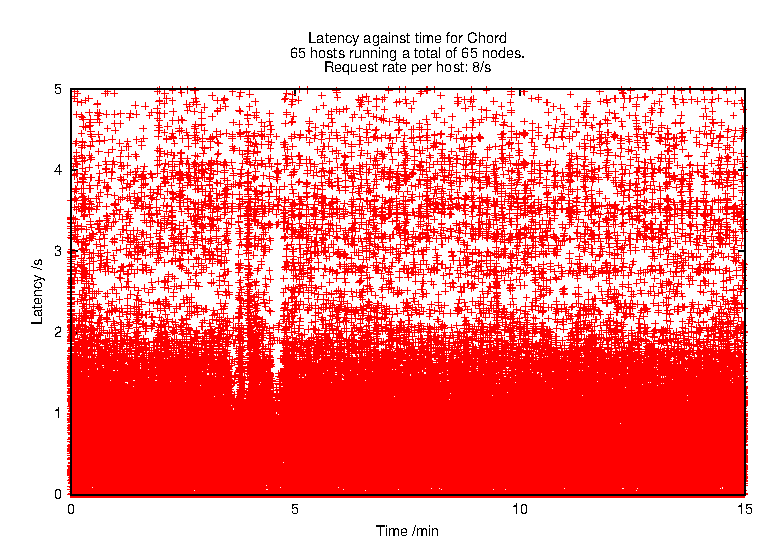
\includegraphics[width=0.9\linewidth]{illustrations/latency_aginst_time_chord.eps}
    \caption{This graph shows how latency vary with time in a 15 minute experimental run of Chord.}
    \label{figLatencyAgainstTime}
  \end{center}
\end{figure}

\begin{figure}[!htbp]
  \begin{center}
    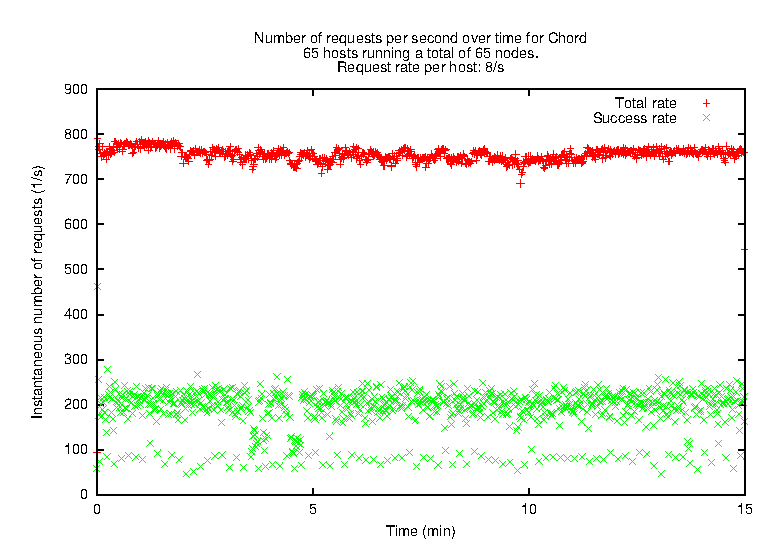
\includegraphics[width=0.9\linewidth]{illustrations/rate_against_time_chord.eps}
    \caption{This graph shows how the request rate and success rate varies over a 15 minute experimental run of Chord.}
    \label{figRateAgainstTime}
  \end{center}
\end{figure}

% * How logging not affect results
During experimental runs I would turn off all functionality not directly needed for serving the requests. This would include turning off the mechanisms that kept the nodes routing state up to date. If a node disappeared during an experiment, nodes contacting it directly would take note of it, but other nodes wouldn't have the node's disappearance reflected in their routing state like they would under normal operation. This might seem somewhat counter-intuitive, but makes sense for my experiments for several reasons.
In my experimental builds of Chord and Pastry I had turned up the rate at which routing information was dissipated through the network to an extreme in order to cut down the waiting time between experimental runs. Since what I wanted to test was the latency of routing requests through the network rather than ancillaries like maintaining the routing state, removing the overhead of keeping the routing state up to date was the right thing to do. This overhead differs between Chord and Pastry, and depends on parameters that would have to be tweaked before using this system in any real world deployment, and therefore would unfavourably affect the test results.

% * How load spread evenly
\mbox{}

To spread the load as evenly as possible across the network of nodes, each search engine host, hosting Distributed Hash Table nodes, would issue requests to the network through its locally hosted nodes.
The keys used in the requests were randomly generated by hashing a combination of the IP-address of the machine issuing the request and a time stamp. This approach gives keys with a nice spread, but results in keys that differ from experimental run to experimental run. While this makes repeatable experiments impossible, it evenly spreads the load between the machines.

% * What constitutes a valid run
Data from experimental runs where a significant number of machines disappeared during the run was discarded.


\section{Results}
Throughout my experiments, a valid request is defined as a request that completes within 5 seconds. By that definition, all other requests are invalid, regardless of if they fail to complete at all, or if they just complete after more than 5 seconds have passed.
% Comment on what is a valid request. And what is considered a failed request
% Findings to comment on:

\subsection{Mean latency and success rate for Chord and Pastry}
In figure \ref{figChordLatency} and \ref{figPastryLatency} you see the latency for different rates and different number of nodes per machine for around 60 machines, shown with 95\% confidence intervals. 

It is noticeable how the latencies for Chord (figure \ref{figChordLatency}) are higher than they are for Pastry (figure \ref{figPastryLatency}), and also how there is less of a correlation between different experimental configurations and the resulting latencies.
For Chord there seems to be a trend showing that the latencies for a fixed number of nodes per host decreases for higher request rates.

In the case of Pastry (figure \ref{figPastryLatency}) we see how the latencies consistently grow larger for increasing total numbers of nodes. Intuitively one would think this is as it should be as the number of nodes involved in any given key-lookup on average should increase proportionally to the logarithm of the number of nodes in the Distributed Hash Table network, but for this set-up with Pastry nodes it is somewhat counter intuitive. The number of hosts the nodes are run on is constant resulting in more nodes per host. One would expect this should let Pastry's proximity heuristic reduce rather than increase the latency as more nodes running on the same physical hosts allow some of the message passes being between nodes with close to no latency.
Unfortunately, these results where performance decreases when more nodes are run on the same hardware agree with the results seen when evaluating the performance improvements given by running multiple nodes on the same host and using the Pastry proximity heuristic (figure \ref{figPastryHeuristic}) presented later in this chapter. 

What we seem to see in figure \ref{figPastryLatency} is that as the number of nodes in the network as a whole grows, the average number of nodes involved in each requests also increases resulting in the inter-node connection latency playing a greater role in routing messages.

\begin{figure}[!htbp]
  \begin{center}
    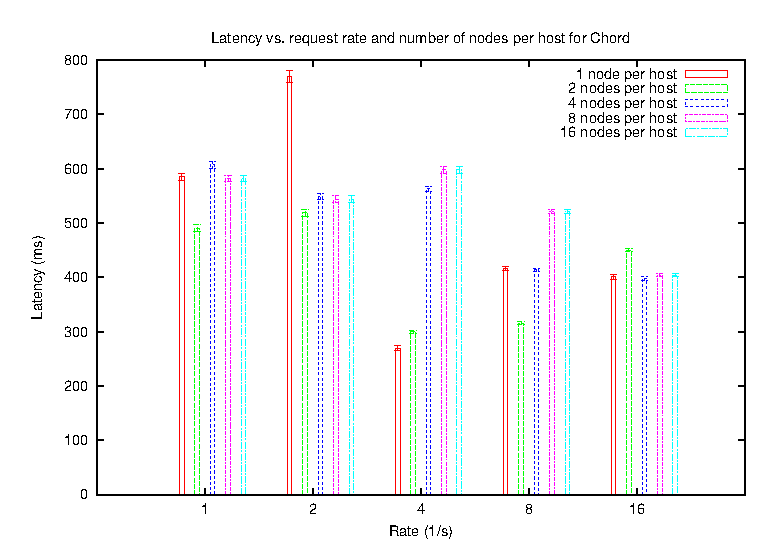
\includegraphics[width=0.9\linewidth]{illustrations/latency_chord.eps}
    \caption{This graph shows latencies for Chord with 95\% confidence intervals for setups of slightly above 60 nodes.}
    \label{figChordLatency}
  \end{center}
\end{figure}

\begin{figure}[!htbp]
  \begin{center}
    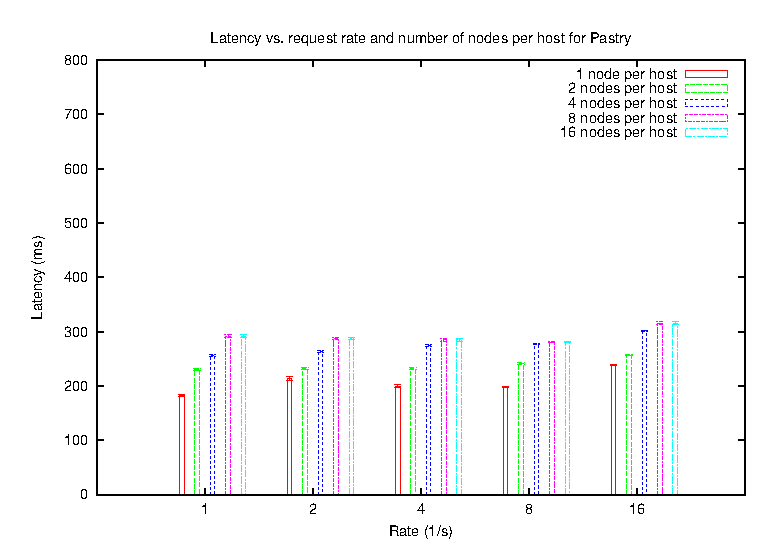
\includegraphics[width=0.9\linewidth]{illustrations/latency_pastry.eps}
    \caption{This graph shows latencies for Pastry with 95\% confidence intervals for setups of slightly above 60 nodes.}
    \label{figPastryLatency}
  \end{center}
\end{figure}

\begin{figure}[!htbp]
  \begin{center}
    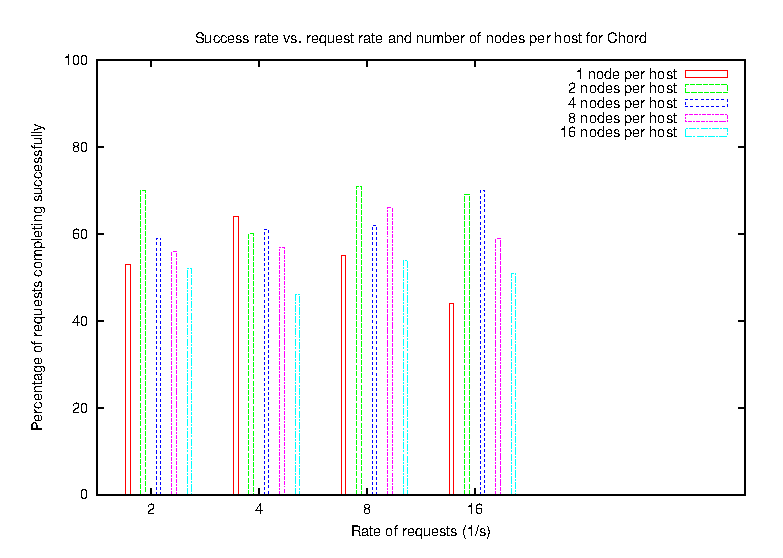
\includegraphics[width=0.9\linewidth]{illustrations/success_rate_chord.eps}
    \caption{This graph shows the percentage of successful requests for different request rates and number of nodes per host for an experimental setup with slightly more than 60 Chord nodes.}
    \label{figChordSuccessRate}
  \end{center}
\end{figure}

\begin{figure}[!htbp]
  \begin{center}
    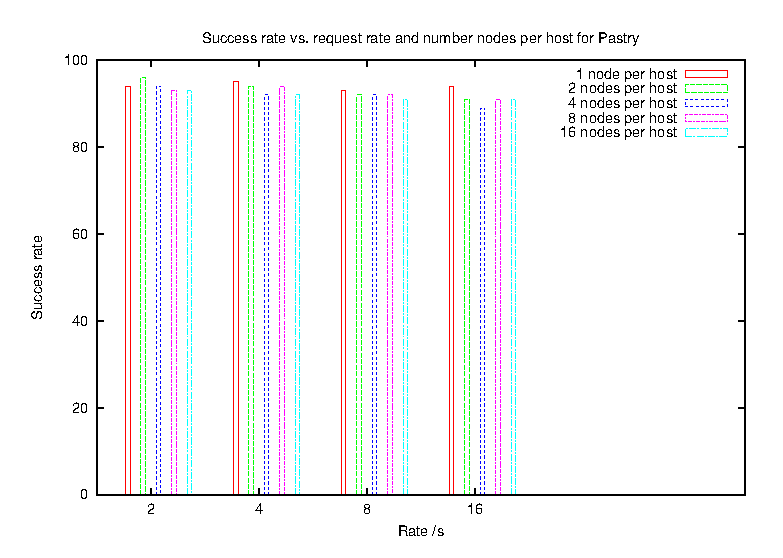
\includegraphics[width=0.9\linewidth]{illustrations/success_rate_pastry.eps}
    \caption{This graph shows the percentage of successful requests for different request rates and number of nodes per host for an experimental setup with slightly more than 60 Pastry nodes.}
    \label{figPastrySuccessRate}
  \end{center}
\end{figure}


The success rate is also dramatically different between Chord (figure \ref{figChordSuccessRate}) and Pastry (\ref{figPastrySuccessRate}). Chord seems to perform better when more than one node is run on the same machine, while Pastry's success rate slightly decreases the more nodes are run on the same physical hardware. It is also worth noting that even at its best, Chord can't compare with the worst case performance of Pastry.

Unfortunately, there is no good explanation for the variations we see within the different configurations for Chord, but it can be explained why Chord, in general, performs so much worse than Pastry.

First, however, I want to discuss how Chord and Pastry behave when pushed to their limits. The cumulative distribution functions for Chord (figure \ref{figChordCDF}) and Pastry (figure \ref{figPastryCDF}) show the fraction of requests succeeding within a certain time. The experiments are run on roughly 60 machines hosting 1 node each. 
For Chord the success rate is only marginally worse for 128 and 64 requests per second per hosts than when there are 16 requests per second per machine. Also rather odd is how the rate of 2 requests per second performs significantly worse than what does the rate of 4 in the case of Chord. I have no good explanations for this behaviour.
For Pastry on the other hand, we see how the success rate gradually drops for extreme rates with Pastry.

It can also be noticed how the cumulative distribution function graph seems to plateau relatively quickly after around twice the average latency. What this tells us is that if a request does not succeed within a relative short window of time, the probability of it still completing successfully is small. This knowledge could be used to set sensible time-out values for lookups.

\begin{figure}[!htbp]
  \begin{center}
    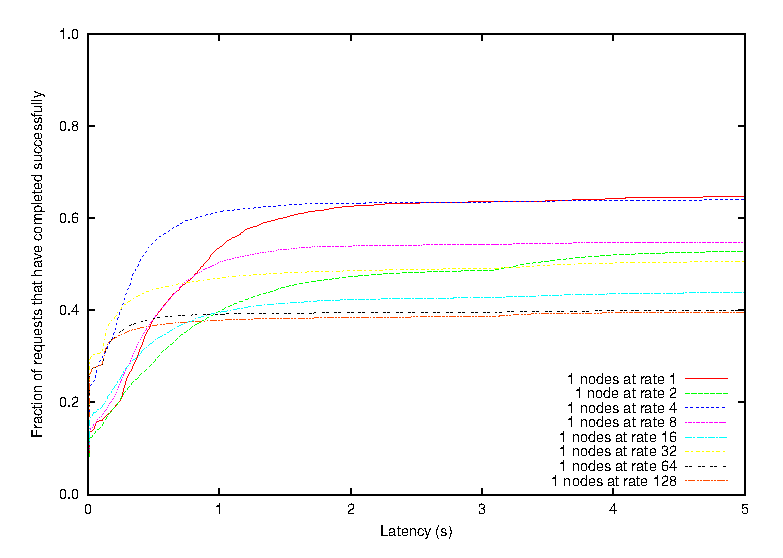
\includegraphics[width=0.9\linewidth]{illustrations/cdf_chord.eps}
    \caption{This graph shows the cumulative distribution function of a request being successful within the first 5 seconds for Chord.}
    \label{figChordCDF}
  \end{center}
\end{figure}

\begin{figure}[!htbp]
  \begin{center}
    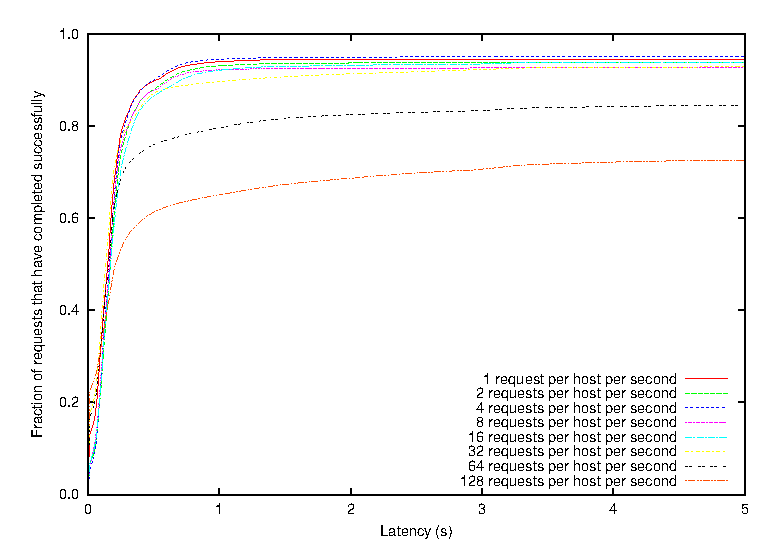
\includegraphics[width=0.9\linewidth]{illustrations/cdf_pastry.eps}
    \caption{This graph shows the cumulative distribution function of a request being successful within the first 5 seconds for Pastry.}
    \label{figPastryCDF}
  \end{center}
\end{figure}

\subsection{Why Pastry performs better that Chord}
The experimental evidence shown so far shows Pastry as superior to Chord both in terms of latency and in the success rate of requests. I will now explain in turn what the causes might be.

\mbox{}

The higher latencies of Chord are the easiest to explain. In figure \ref{figChordNumNodes} and \ref{figPastryNumNodes} you see how many nodes are involved in key lookups for Chord and Pastry respectively. It is clear from the graph that the average number of nodes involved in a key lookup are greater for Chord than for Pastry. If one multiplies the average time it takes two randomly chosen nodes to connect with the number of nodes involved in a key lookup, it should be clear that a Chord lookup should take longer if the only thing one is accounting for is the latency of the routing. Additionally, Pastry uses a heuristic when routing, favouring nodes closer by, which also affects the latency as each routing step is likely to take less time for Pastry than it does for Chord. I will shortly discuss the impact of the proximity heuristic in Pastry.

Whether the higher number of routing steps for Chord is an implementation specific bug or something inherent to the Chord algorithm is unclear. It is possible that the difference would become less significant for larger networks of nodes. Unfortunately, this is not something I was able to test given the infrastructure available.

\begin{figure}[!htbp]
  \begin{center}
    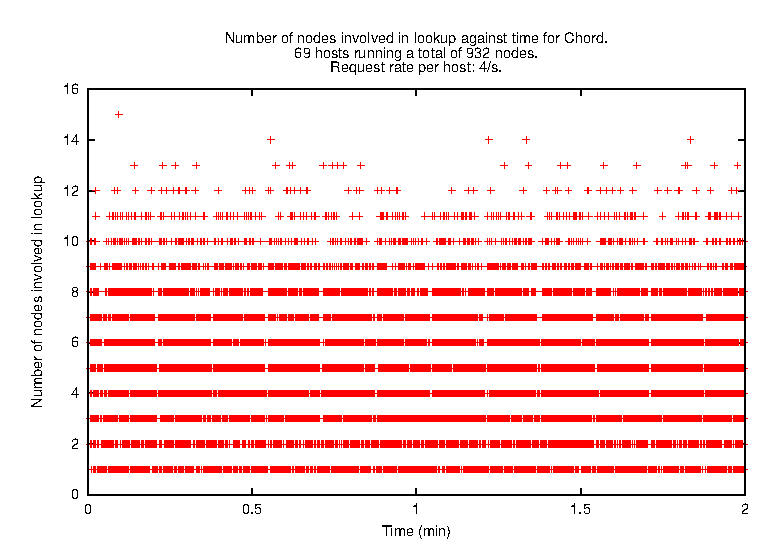
\includegraphics[width=0.9\linewidth]{illustrations/nodes_against_time_chord.eps}
    \caption{This graph shows the number of nodes involved in a key lookup in a particular experimental run for Chord.}
    \label{figChordNumNodes}
  \end{center}
\end{figure}

\begin{figure}[!htbp]
  \begin{center}
    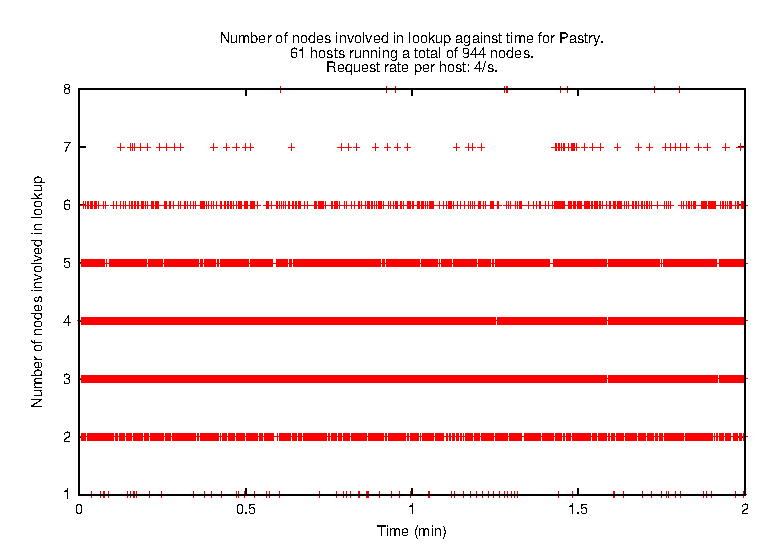
\includegraphics[width=0.9\linewidth]{illustrations/nodes_against_time_pastry.eps}
    \caption{This graph shows the number of nodes involved in a key lookup in a particular experimental run for Chord.}
    \label{figPastryNumNodes}
  \end{center}
\end{figure}

\mbox{}
Now that we have an idea of why the latency might be higher for Chord than for Pastry, let me explain why the failure rate is higher as well.

First, let us recall how Chord and Pastry perform their routing.
In Chord, the node that wants to lookup a key (the requester) asks the node closest to the key that it knows about if it knows about other nodes closer to the target key. It then asks the node it gets returned the same question, and the pattern continues until it finds the node immediately preceding the key. Its successor is the target node responsible for the key.

Pastry follows a different approach. When a requesting node sends a message addressed to a key it forwards the message to the node it knows about that is closest to the message key. Where it differs from the Chord approach is that the requester hands over the responsibility for having the message forwarded onwards to its destination to the node it itself forwarded it to.

Now lets consider what happens when something goes wrong.
In figure \ref{figureChordFailedLookup}, we see what happens when Chord node A gets returned node D as the next hop node from B. D is not accessible and the lookup fails. If A retries the routing step, B again returns D, unless it has already noticed that D is inaccessible.

In the case of Pastry (figure \ref{figurePastryFailedLookup}) node B becomes responsible for routing the request forward towards the target node. Upon realising node D is unavailable it routes it to the next closest node it knows about, in this case C. Node C happens to know about a node closer to the target than D, and this way we managed to route around the unavailable node.

There are workarounds for improving Chord's routing performance. One would be for the requesting node A to inform node B about node D's death upon retrying to route the message. An alternative could also have been for node A to try to route the request through another intermediate node before D, but in this case we are not guaranteed that this intermediate node will not also return D.
A third approach could be to look up D's predecessor, and then use that node in the same role previously filled by B. None of these methods have been used in my implementation as they would extend the core Chord routing algorithm and therefore skew the comparison in Chord's favour.
For that matter, it might be that the solution is as simple as leaving the mechanism for maintaining routing state on for the duration of the experiments, but initial experiments run before I decided to turn off the routing state maintenance during experiments do not seem to indicate this.

\begin{figure}[!htb]
\begin{center}
  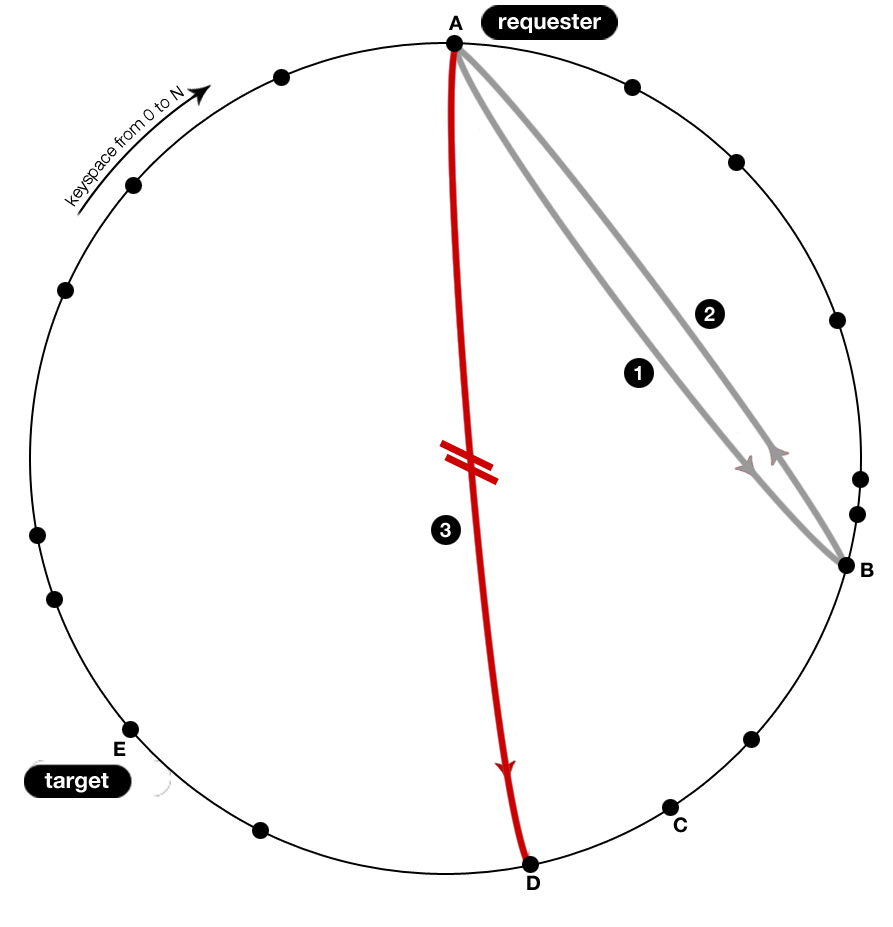
\includegraphics[width=0.9\linewidth]{illustrations/ChordRoutingFailed.png}
  \caption{The illustration shows what happens when routing fails in Chord. We see how when node A gets the unavailable node D returned from B, it is stuck and the routing fails.}
  \label{figureChordFailedLookup}
\end{center}
\end{figure}

\begin{figure}[!htb]
\begin{center}
  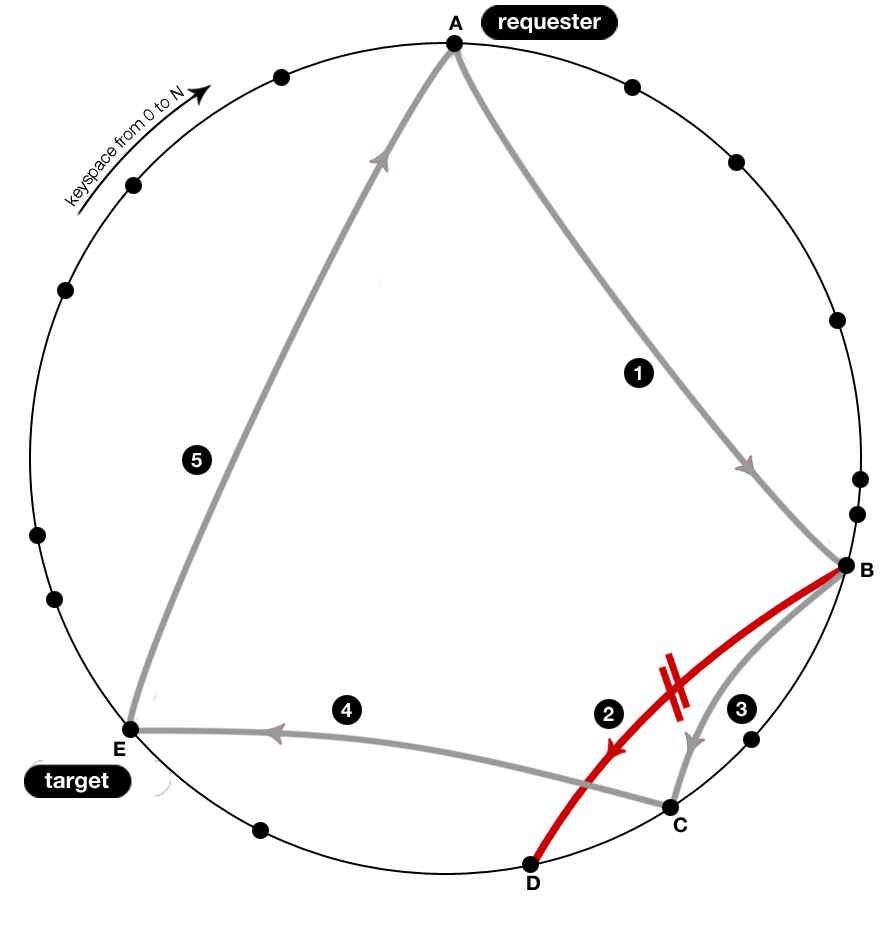
\includegraphics[width=0.9\linewidth]{illustrations/PastryRoutingFailed.png}
  \caption{The illustration shows how Pastry deals with node failure during message routing. The unavailable node D is routed around by node B to get to the target node.}
  \label{figurePastryFailedLookup}
\end{center}
\end{figure}

% * Why is Chord so much slower than Pastry?
% * Why does Chord has such a low yield rate compared to Pastry
% * How much can we conclude from the numbers?

\section{Effect of Pastry routing heuristics}
% * What effect does the Pastry routing heuristics have on the performance
In this section I look at how the heuristics used in my implementation of Pastry affect the routing performance. 

I have sampled the latencies from Pastry in a small set of different configurations with the heuristic enabled and then with the heuristic turned off. Please note that this is nothing but a very limited sample and by no means an exhaustive evaluation of the heuristic, or heuristics in general. One should not try to generalize the findings based on this data or read it as valid for anything but the sampled configurations.

The following configurations were sampled:
\begin{itemize}
\item 10 machines running 1 node each
\item 10 machines running 5 nodes each
\item 50 machines running 1 node each
\item 50 machines running 16 nodes each
\end{itemize}

The choice of configurations was made for the following reason.
I wanted to see how expanding the network by adding additional machines at new geographical locations affect the latency.
I also wanted to see how running 50 nodes across a few machines compared to running 50 nodes on 50 different machines. Lastly, I wanted to see how the heuristic behaved in the more extreme case with a larger network with relatively large cliques of nodes close to each other.

The results seen in figure \ref{figPastryHeuristic} partly show what one would expect; that the heuristic improves the routing performance.

\begin{figure}[!htb]
  \begin{center}
    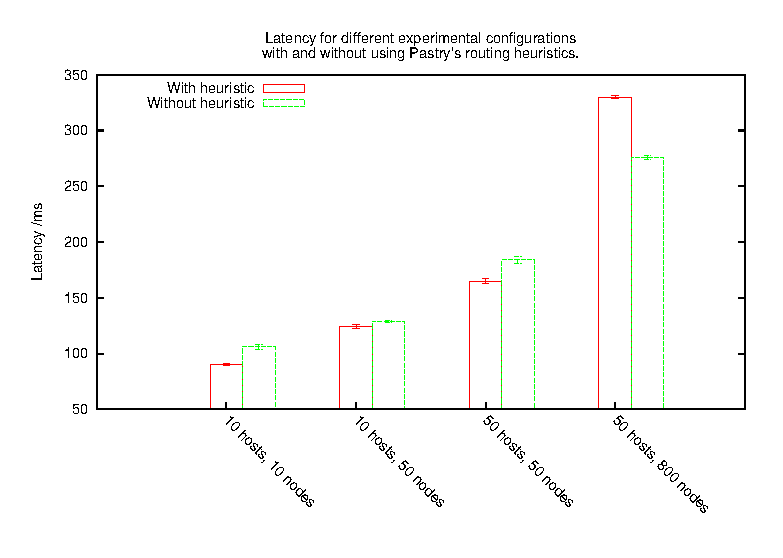
\includegraphics[width=0.9\linewidth]{illustrations/pastry_heuristic.eps}
    \caption{Latencies for Pastry with and without the routing proximity heuristic activated. Shown with 95\% confidence intervals.}
    \label{figPastryHeuristic}
  \end{center}
\end{figure}

As one would expect, the heuristic allowing nodes to preferentially route to geographically closer nodes for the most part improved the performance substantially. In the two cases where only 1 node was run per host we see a 15\% and 10\% gain for the 10 machine and 50 machine cases respectively.
Quite surprisingly, the cases where multiple nodes are located on the same machine, scenarios where I would have expected the heuristic to shine, perform less well. In the case where 50 nodes are spread over 10 hosts we only see a 4\% performance gain when using the heuristic, and in the case where 50 machines run 16 nodes each, the performance drops by 20\% when the heuristic is being used.

The heuristic is only calculated when nodes are added to the routing table during the routing state stabilization phase, and should therefore not affect the routing performance locally within a node.
A reason could be that while the Pastry paper \cite{pastry} suggests nodes use an expanding ring multi-cast to find other Distributed Hash Table nodes to connect to, which would result in the node automatically getting to know all its nearby neighbour-nodes, I made all nodes contact the central control hub in order to get nodes to connect to. The central control hub does not take node proximity into account and as a result a node might not know about all the other nodes living on the same physical hardware. The reasoning behind this design decision originally came from the insight that most nodes would live in completely separate physical networks and that multicast messages would never be able to get from one node to the next, but making that decision I failed to account for multiple hosts living on the same machine.
This is a weakness in my implementation rather than in Pastry itself, and something that would be interesting to look into for the future. While multicast might still not be an ideal solution, it would be interesting for Pastry nodes that are not the first node on a machine to use other nodes hosted on the same hardware as their entryway into the Distributed Hash Table network.
Yet this does not explain why the performance is better without the heuristic as the nodes join the network the same way in both cases.

It might be that the heuristic of hop count in the underlying network is just suboptimal and that a pure latency based heuristic should be used instead.
These results highlight the importance of relying on metrics when making design decisions rather than blindly implementing performance enhancements in the faith that optimisations are always for the better.

Less interesting, but reassuring non the less, is that the latency grows with increasing number of nodes in the network, just like one would expect. Unfortunately this dataset is too limited to give a general measure of how the latency grows with the network size.

\section{Cost of using link records}
\label{sec:costOfLinkRecords}
As introduced in the preparation chapter, my implementation uses \emph{link records}, records pointing to full \emph{profile records}, in order to provide predictive and fuzzy search.

I will now evaluate how this affects the storage requirements of the Distributed Hash Table network, and also the number of key lookups that need to be done for a particular search.

First, let us look at the how the storage requirements are affected.
I have a sample of 170 million names taken from Facebook. This sample might not follow the distribution of names in the real world, but most certainly quite accurately models the kind of names people give themselves in online social networks.

Based on \emph{link records} for 20 million names, I can with 99\% confidence say that the social network population mean name would require 5.322 $\pm$ 0.001 link records. I can also say that the population mean average length of a name is 14.959 $\pm$ 0.002 characters.

If each link record consists of a user's full name, the key of the \emph{profile record} and the key of the \emph{link record} itself, then the storage requirement of each \emph{link record} is roughly 55bytes, or 300bytes per \emph{profile record}, assuming each character is stored using 8 bits.
In my opinion this is not an issue.

Now, let us consider the number of extra lookups that would be required for a predictive search using link records. Table \ref{tableIndianName} and table \ref{tableAmericanName} show the amount of new link records that have to be downloaded when the user adds an extra character to the name being searched for and how much space these link records take. The second and third leftmost columns show the amount of link records given the link records currently used, where link records are generated for each additional three characters in a user's name. The subsequent columns show how many link records there would be if link records were generated for each additional 4, 5 and 6 characters in a users name.
The link records are generated from a sample of 60 million names evenly distributed in the bag of names taken off of Facebook.

\begin{table}[!htb]
\caption{Number of link new link records per additional character in the search term Archaya Pruedsakaran and the size of the link records for the cases where link records are generate for each additional 3, 4, 5 and 6 characters in a name. Green cells indicate that one of the new link records points to the profile record we are looking for.}
\begin{center}
\scriptsize{
  \begin{tabular}{ | l | r | r | r | r | r | r | r | r | }
    \hline                       
    \multicolumn{9}{|l|}{\textbf{Atchaya Pruedsakaran}} \\ 
    \hline                       
    \hline  
    & \multicolumn{2}{l|}{3 char} & \multicolumn{2}{l|}{4 char} & \multicolumn{2}{l|}{5 char} & \multicolumn{2}{l|}{6 char}  \\
    Query & \# links & size /MB & \# links & size /MB & \# links & size /MB & \# links & size /MB  \\
    \hline  
    A                         & 163600 & 46.81 & 163600 & 46.81 & 163600 & 46.81 & 163600 & 46.81 \\
    \hline                   
    At                        & 4357 & 1.25 & 4357 & 1.25 & 4357 & 1.25 & 4357 & 1.25 \\
    \hline                   
    Atc                       & \cellcolor{green} 3966 & 1.13 & 112 & 0.03 & 112 & 0.03 & 112 & 0.03 \\
    \hline                   
    Atch                      & 38 & 0.01 & \cellcolor{green} 3716 & 1.06 & 38 & 0.01 & 38 & 0.01 \\
    \hline                   
    Atcha                     & 106 & 0.03 & 106 & 0.03 & \cellcolor{green} 792 & 0.23 & 106 & 0.03 \\
    \hline                   
    Atchay                    & \cellcolor{green} 24 & 0.01 & 2 & 0.00 & 2 & 0.00 & \cellcolor{green} 24 & 0.01 \\
    \hline                   
    Atchaya                   & \cellcolor{green} 15 & 0.00 & \cellcolor{green} 15 & 0.00 & \cellcolor{green} 15 & 0.00 & \cellcolor{green} 15 & 0.00 \\
    \hline                   
    Atchaya P                 & 45741 & 13.09 & 45741 & 13.09 & 45741 & 13.09 & 45741 & 13.09 \\
    \hline                   
    Atchaya Pr                & 175 & 0.05 & 175 & 0.05 & 175 & 0.05 & 175 & 0.05 \\
    \hline                   
    Atchaya Pru               & \cellcolor{green} 15091 & 4.32 & 55 & 0.02 & 55 & 0.02 & 55 & 0.02 \\
    \hline                   
    Atchaya Prue              & 244 & 0.07 & \cellcolor{green} 2372 & 0.68 & 244 & 0.07 & 244 & 0.07 \\
    \hline                   
    Atchaya Prued             & 0 & 0.00 & 0 & 0.00 & \cellcolor{green} 5 & 0.00 & 0 & 0.00 \\
    \hline                   
    Atchaya Prueds            & \cellcolor{green} 2 & 0.00 & 0 & 0.00 & 0 & 0.00 & \cellcolor{green} 2 & 0.00 \\
    \hline                   
    Atchaya Pruedsa           & 0 & 0.00 & 0 & 0.00 & 0 & 0.00 & 0 & 0.00 \\
    \hline                   
    Atchaya Pruedsak          & 0 & 0.00 & \cellcolor{green} 2 & 0.00 & 0 & 0.00 & 0 & 0.00 \\
    \hline                   
    Atchaya Pruedsaka         & \cellcolor{green} 2 & 0.00 & 0 & 0.00 & 0 & 0.00 & 0 & 0.00 \\
    \hline                   
    Atchaya Pruedsakar        & 0 & 0.00 & 0 & 0.00 & \cellcolor{green} 2 & 0.00 & 0 & 0.00 \\
    \hline                   
    Atchaya Pruedsakara       & 0 & 0.00 & 0 & 0.00 & 0 & 0.00 & 0 & 0.00 \\
    \hline                   
    Atchaya Pruedsakaran      & \cellcolor{green} 2 & 0.00 & \cellcolor{green} 2 & 0.00 & \cellcolor{green} 2 & 0.00 & \cellcolor{green} 2 & 0.00 \\
    \hline  
  \end{tabular}
}
\end{center}
\label{tableIndianName}
\end{table}


\begin{table}[!htb]
\caption{Number of link new link records per additional character in the search term Brad Catron and the size of the link records for the cases where link records are generate for each additional 3, 4, 5 and 6 characters in a name. Green cells indicate that one of the new link records points to the profile record we are looking for.}
\begin{center}
\scriptsize{
  \begin{tabular}{ | l | r | r | r | r | r | r | r | r | }
    \hline                       
    \multicolumn{9}{|l|}{\textbf{Brad Catron}} \\ 
    \hline                       
    \hline  
    & \multicolumn{2}{l|}{3 char} & \multicolumn{2}{l|}{4 char} & \multicolumn{2}{l|}{5 char} & \multicolumn{2}{l|}{6 char}  \\
    Query & \# links & size /MB & \# links & size /MB & \# links & size /MB & \# links & size /MB  \\
    \hline  
    B                & 73400 & 21.00 & 73400 & 21.00 & 73400 & 21.00 & 73400 & 21.00 \\
    \hline
    Br               & 434 & 0.12 & 434 & 0.12 & 434 & 0.12 & 434 & 0.12 \\
    \hline
    Bra              & \cellcolor{green} 956906 & 273.77 & 475 & 0.14 & 475 & 0.14 & 475 & 0.14 \\
    \hline
    Brad             & \cellcolor{green} 157479 & 45.06 & \cellcolor{green} 305181 & 87.31 & \cellcolor{green} 157479 & 45.06 & \cellcolor{green} 157479 & 45.06 \\
    \hline
    Brad C           & 91473 & 26.17 & 91473 & 26.17 & 91473 & 26.17 & 91473 & 26.17 \\
    \hline
    Brad Ca          & 3800 & 1.09 & 3800 & 1.09 & 3800 & 1.09 & 3800 & 1.09 \\
    \hline
    Brad Cat         & 4\cellcolor{green} 63292 & 132.55 & 22172 & 6.34 & 22172 & 6.34 & 22172 & 6.34 \\
    \hline
    Brad Catr        & 2 & 0.00 & \cellcolor{green} 13414 & 3.84 & 2 & 0.00 & 2 & 0.00 \\
    \hline
    Brad Catro       & 30 & 0.01 & 30 & 0.01 & \cellcolor{green} 857 & 0.25 & 30 & 0.01 \\
    \hline
    Brad Catron      & \cellcolor{green} 748 & 0.21 & \cellcolor{green} 703 & 0.20 & \cellcolor{green} 703 & 0.20 & \cellcolor{green} 748 & 0.21 \\
    \hline  
  \end{tabular}
}
\end{center}
\label{tableAmericanName}
\end{table}

What we see is that there are a lot of link records for 1 character search queries (163k for \emph{a} and 73k for \emph{b}) and in the case of link records generated for each 3 or 4 additional characters also when the query is as long as the length at which the first link record is generated. Short common names like Brad also generate a lot of link records.

What gives this approach some hope is that there are significantly fewer link records when longer name fragments are used for generating link records, and also in the cases where we generate link records for each 3 additional characters, there seem to be much less link records for the second link record generated for a name.

Caching link records for all character combinations up to 3 characters could be a possibility, but back of the envelope calculations based on the numbers presented indicate that this would require several gigabytes worth of local caches per host, and probably more than that if the system was also to accommodate non-latin character sets. While possible, this might be a bit too much to ask of the independent distributed online social networks.

Other promising performance enhancements like adding query length thresholds and compressing the link record data are discussed and evaluated in Appendix \ref{sec:appendixLinkRecords}.

\section{Utility of Chord and Pastry as back end data stores for a search engine}
% Conclude
% * Does it work for search engine?
In its current raw form, Chord is not really a viable data store for any application. Its high and variable latency, although undesirable, is something one could live with, if the key lookups would not have such a high failure rate.
Pastry on the other hand proves a quite efficient key-value store, even in highly distributed environments. Its combination of high success rates and consistently low key lookup latencies and gradual degradation in performance under high load are all desirable properties.

If one uses a combination of caching link records at the search servers, add a query length threshold before which no requests are made to the search network, and make the search servers more capable of judging the relevance of link records, in addition to compressing and minimizing the size of link records, I think key-value stores could quite efficiently be used as the back end data store for a search engine. Especially considering the benefits Distributed Hash Tables bring like built in load balancing, fault tolerance and predictable and scalable performance.

\mbox{}

In this chapter we have seen how my implementation of Pastry outperforms my implementation of Chord both in terms of latency and key lookup success rate.
We have also discovered how the proximity heuristic used in routing by Pastry quite counter intuitively does not always yield performance improvements, and have understood the importance of relying on metrics rather than intuition when evaluating performance.

We also looked at the impact using link records has on the amount of data that needs to be stored in the network and the number of link records loaded during two sample searches.

Finally we concluded that with some optimizations in the search server, Distributed Hash Tables can work quite well as the data store for a Distributed Search engine of the particular kind I have proposed.
